\section{Preliminaries}

\subsection{Concepts}
We model the database as a large relation $DB$. This table contains two types of
columns: the dimensions $D_0, \ldots, D_d$ and the target columns $T_0, \ldots,
T_t$.  Note that this view is logical: we are oblivious to the physical
structure of the data. Furtermore, we assume that each dimension $D_k$ has
several variants $D_k^p$, where $p$ is the level of precision.  If the
dimensions are explicitely organized as a hierarchy (e.g.  Country > State >
City), then $p$ describes the level in the hierarchy ($D_k^1$ represents
Country). If not, $D_k^p$ describes a binned version of $D_k$, with $2^p$ bins
of equal size.

\begin{figure}[t!]
\centering
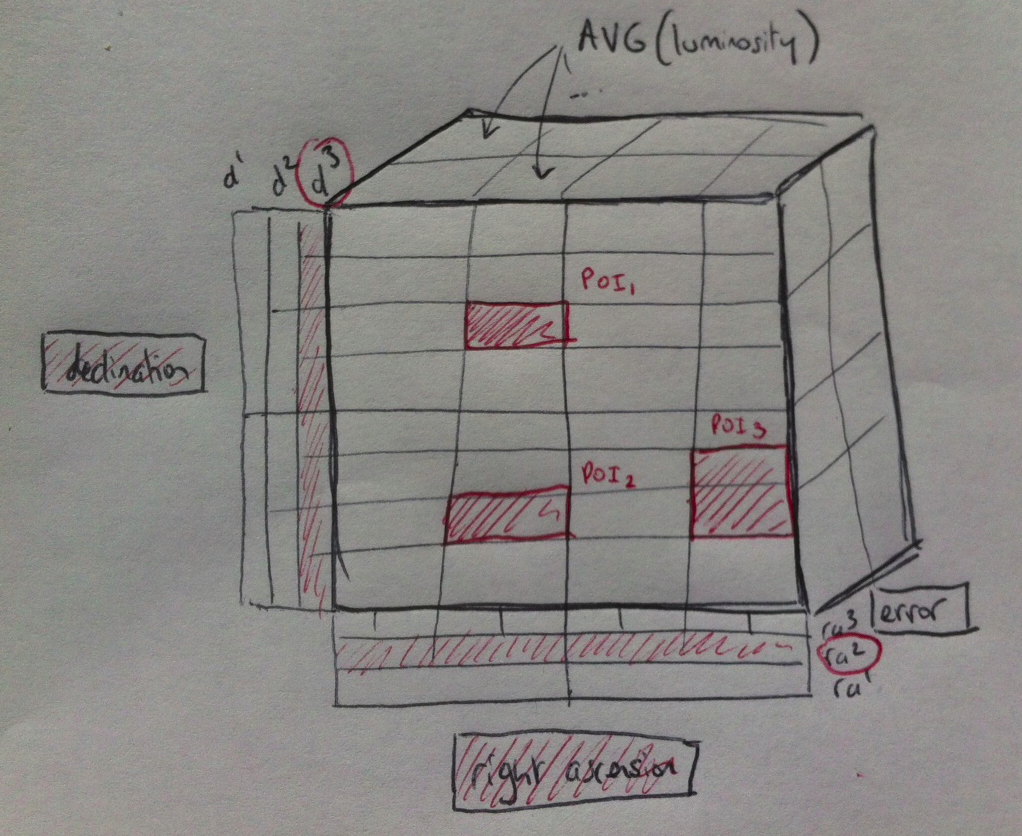
\includegraphics[width=\columnwidth]{images/cube}
\caption{Example of recommendation}
\label{cube}
\end{figure}

Given a hypercube $DB$, Claude's aim is to generate a ranked set of
\textbf{suggestions}.  Each suggestion contains two elements: a \textbf{view}
and a set of \textbf{points of interest} (POI). A view is a set of dimensions.
A point of interest is a selection on these dimensions. It reveals a region
in which the target has an ``usual'' distribution.  We illustrate these
concepts with Figure \ref{cube}. Our example database describes light sources
with three dimensions: \texttt{right ascension}, \texttt{declination} and
\texttt{error}.  The first two describe a source's position. The thrid one
describes the measurement errors. Our aim is to study the luminosity of these
sources. Claude's recommendations are highlighted in red. It suggests a view
based on \texttt{right ascension}, and \texttt{declination}, with precision
levels 2 and 3 respectively. We see that the view is a SQL query with the
following structure:
\begin{verbatim}
SELECT   D0, ... , Dn , AVG(M0), ... , AVG(Mm)
FROM     T
GROUPBY  D0, ... , Dn
\end{verbatim}
Claude's job is to pick the $n$ distinct variables $\texttt{D0} \ldots
\texttt{Dn}$. Each of these variables represents one dimension and its
precision level.  Once Claude has chosen a view, it must explain \emph{why} it
has chosen this view.  This is the role of POIs. In Figure \ref{cube}, Claude suggests
four POIs. We can express them in SQL as follows:
\begin{verbatim}
SELECT   AVG(M0), ... , AVG(Mm)
FROM     T
WHERE    D0 BETWEEN l0 AND h0
 AND     ...
 AND     Dn BETWEEN ln AND ln
\end{verbatim}
The variables $\texttt{D0} \ldots \texttt{Dn}$ come from the previous step. The
challenge is to set the ranges $\texttt{[l0,h0]}, \dots \texttt{[ln,hn]}$.


\subsection{Significant suggestions}
\begin{figure}[t!]
\centering
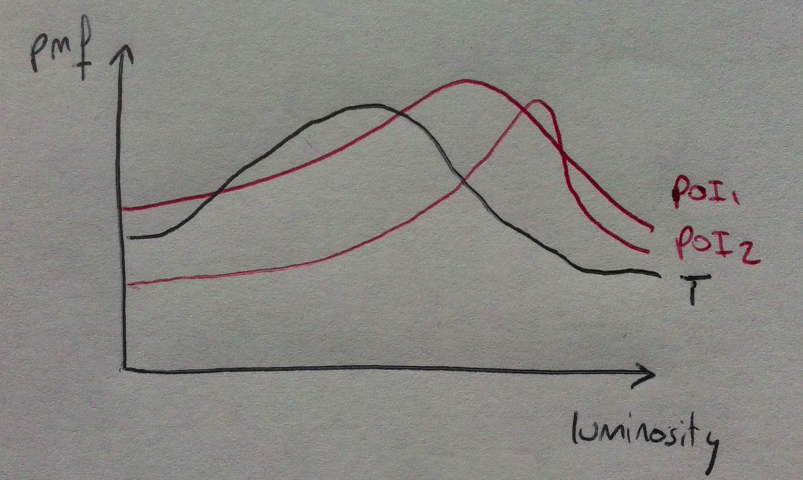
\includegraphics[width=\columnwidth]{images/poi}
\caption{The POIs have unusual distributions}
\label{poi}
\end{figure}

We defined our search space: we want to suggest views and POIs. We now present
how to recognize the interesting ones. We describe the $t$ target columns with
a random vector $T$.  We represent each  dimension $D_k^p$ by a random
variable $D_k$ (for now we abstract the level of precision).

First let's explain how to choose the views.  Intuitively a view is worth
consering if its columns are ``related'' to the target.  We model this
relationship with statistical dependency. \emph{We assume that a view is
interesting if there exists some statistical dependency between its variables
and the target}. In our framework, the more dependent the dimensions are to the
target, the more interesting the view is. We can formalize this statement 
wihtout loss of generality with Mutual Information \cite{cover2012elements}:

\begin{definition}
Consider a view $V$, based on the variables $D_0, \ldots, D_n$. The variable
$T$ describes the target variables.  Let $I$ denote the \emph{Mutual
Information}. We define the \textbf{interestingness} of $V$ as follows: $\alpha(V) =
I(D_0, \ldots, D_n ; M)$.
\end{definition}

Note that this definition d
The next step is to \emph{describe} this influence with the POIs. The POIs
contain tuples for which the measure have an ``unusual'' distribution.
Consider Figure \ref{poi}. The curves show the probability mass function of the
luminosity for three sets: the whole database $DB$, $POI_1$ and $POI_2$. We
observe that the sets $POI_1$ and $POI_2$ deviate a lot from the rest of the
database.  Therefore, we consider them as significant. We quantify this
observation with the Kullback-Leibler divergence:

\begin{definition}
Consider a random variable $C$, defined over the cells of a view.  The variable $(M |
C=c)$ describes the measures for all the tuples in a given cell $c$.  We define the
\textbf{signifiance} of $c$ as follows: $\sigma(c) = KL( \Pr(M | C=c) \|
\Pr(M)  )$
\end{definition}

Claude's aim is to recommend high impact queries, and a few highly meaningful
cells. As a matter of fact, these two notions are tightly related.

\begin{lemma}
Let $Q$ denote a view. The set $\mathcal{C}_Q$ contains all its cells. We
observe the following relationship:
\[
    \alpha(Q) = \mathbb{E}_{c \in \mathcal{C}_Q} \{ \sigma(c) \}
\]
\end{lemma}

\begin{proof}
By definition of the KL distance, we have: $I(C,M) = \mathbb{E}_C \{ KL( \Pr(M
| C) \| \Pr(C) ) \}$. Observe that the variable $C$ is equivalent to $D_0,
\ldots , D_n$. We derive the final lemma from the definitions of impact and signifiance.
\end{proof}

This lemma is simple but powerful. It shows that impact and signifiance are
``two sides of the same coin'': the impact of a query is exactly equal to the
average signifiance of its cells.  Therefore, we can use the terms impact and
signifiance interchangeably to characterize \emph{suggestions} (recall that a
suggestion contains both the view and its POIs).

\begin{definition}
Let $S=(V, \{c_0, \ldots, c_r\})$ describe a suggestion. The
\textbf{signifiance} (alternatively, \textbf{impact}) of $S$ is the average
signifiance of $V$'s cells.
\end{definition}

\begin{figure}[t!]
\centering
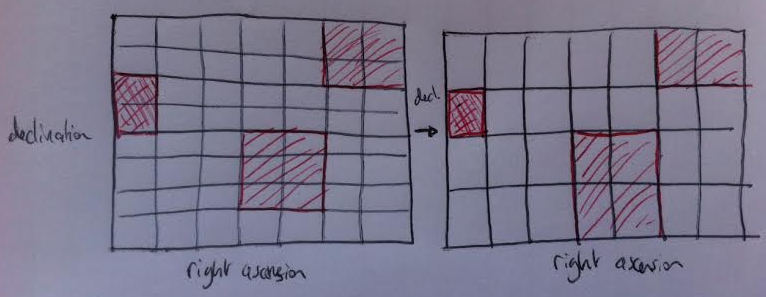
\includegraphics[width=\columnwidth]{images/precision}
\caption{Adaptive drill-up}
\label{precision}
\end{figure}

We have almost all the elements necessary to characterize ``good'' queries.
The only thing missing is the precision level. At which granularity should we
present the suggestions? More bins give more precision. However, a view with
too many cells is overwhelming. We decided to eliminate this problem with a
simple two-step heuristic.  During the first step, we merge all the adjacent
POIs for the highest level of precision. Then, we reduce the grid granularity
(``drill-up'') until each cell is wide enough to contain the smallest
aggregate. We illustrate this process in Figure \ref{precision}.


\subsection{Problem statement and solution overview}

We are now ready to formulate our problem:
\begin{problem}
Consider a hypercube $T$ and a triplet $(q, n, r)$. A \emph{suggestion}
contains one \emph{view} and $r$ regions. A view is a set of $n$ variables.
Find the top $q$ most significant suggestions.
\end{problem}

To solve this problem, Claude operates in two steps. First, it detects $q$ high
impact sets of columns.  We call this step \emph{column search}.  Then comes
the \emph{POI dectection} step. In practice, our top $q$ strategy can generate
redundancy. We tackle this problem with an optional \emph{refinment} step.  We
exploit advances in information theory (KRIMP) to find the most meaningful
suggestions.


\section{Base algorithm}

\subsection{Column Search}
The aim of this phase is identify the $q$ most significant sets of variables.
To understand how Claude operates, we introduce an alternative formulation of
signifiance.

\begin{lemma}
(Chaine Rule) Consider a view $Q$. Let $D_Q$ represent the joint distribution of
its variables, and let $M$ describe the measures of interest. For any variable $D$: 
$$
    \sigma(Q \cup \{D\}) = \sigma(Q) + I(D ; M | D_Q)
$$
\end{lemma}
\begin{proof}
This lemma is a classic result of information theory \cite{cover2012elements}.
\end{proof}

Thanks to this lemmas, we can explore our candidate space with level-wise
search.  First, we enumerate all the sets of exactly one columns. If $d$ is the
dimensionality of the hypercube,  we obtain $d$ candidates. From this set, we
obtain all the sets of two columns. Our new candidate set contains
$\binom{d}{2}$ items (the order does not matter).  We reiterate the
operation until we have $\binom{d}{n}$ sets of $d$ variables. 

Obivoulsy, this procedures does not scale well with $d$. However, $d$ is
limited in practice. It cannot exceed the number of dimensions that a user can
visualize (typically, less than five). Also, we can prune the search space.
The \emph{apriori} property does not appy to our case [to be
confirmed]. However, we can use the following bounds: 

\begin{lemma}
\label{lem:bounds}
Given a view $Q = \{C_0, \ldots , C_i, C_{i+1}, \ldots, C_n\}$:
\begin{align}
    \sigma(Q)  & \geq \sigma(C_0, \ldots , C_i) \label{bound1}\\
     \sigma(Q) & \leq \sigma(C_0, \ldots , C_i) + H(C_{i+1}, \ldots, C_n) \label{bound2}\\
               & \leq \sigma(C_0, \ldots , C_i) + H(C_{i+1}) + \ldots + H(C_n) \label{bound3}
\end{align}
\end{lemma}

\begin{proof}
Cf. appendix.
\end{proof}

Let $\sigma_i$ represent the q\textsuperscript{th} highest significance
obtained at step $i$. Similarly, $\sigma_n$ representd the
q\textsuperscript{th} highest significance at step $n$. Equation \ref{bound1}
states that $\sigma_n \geq \sigma_i$. Thanks to this property, we can reduce
the search space. Consider a candidate $Q$ at step $i$. If we can predict that its
signifiance will never exceed $\sigma_i$, then we can safely discard it.

We can anticipate $Q$'s best possible performance with Equations \ref{bound2}
and \ref{bound3}. Equation \ref{bound2} is the tightest bound. However, it
requires the expensive joint distribution $C_{i+1}, \ldots, C_n$.  In some
cases, we can ``recycle'' it from previous steps: if the view $C_{i+1}, \ldots
,C_n$ is in the candidate set, it means that we already computed it.
If we cannot recycle, we use the looser bound of Equation
\ref{bound3}, or a hybrid form.



\subsection{POI detection}

We detect POIs with beam search.  One subtelty: instead of binning,
we can directly exploit the hierarchy of dimensions in the
database. We explore the highest level first (Continent), then we refine
progressively (Country, City, etc...).


\section{Eliminating redundancy}

We run KRIMP on the result set to get the most meaningful queries.


\section{Faster column search}

The idea here is to cheat. We make a very naive assumption:
\[
\begin{split}
    \sigma(Q \cup \{D_n\}) & = \sigma(Q) + I(D_n ; M | D_0, \ldots, D_{n-1})\\
                           & \approx \sigma(Q) + I(D_n ; M | D_{n-1})
\end{split}
\]

From there, we build a faster algorithm. There may be some connection with
Chow-Liu trees - to be investigated.



\section{Real-life example: radio astronomy}

The aim here is to showcase Claude with a real life use case: finding
transients in an astronomical database. Here, the database represents several
thousands light sources (e.g., stars). The measure of interest is a statistic,
which describes how much the sources deviate from some physical model. Higher
is better.


\section{Experiments}
